\newpage

\genHeader
\subsection{Install our extension for Enterprise Architect}

Enterprise Architect (EA) is a visual modelling tool that supports the Unified Modelling Language (UML) and a host of other modelling languages.
EA is not only affordable but also quite flexible, and can be extended via \emph{extensions} to support new modelling tools -- such as eMoflon!

\begin{stepbystep}
\item Download\hypertarget{installEA vis}{} EA for Windows from \linkto{http://www.sparxsystems.com/} to get a free 30 day trial and follow
installation instructions (\Cref{enterpriseArchitextHomepage}).

\begin{figure}[htbp]
	\centering
  	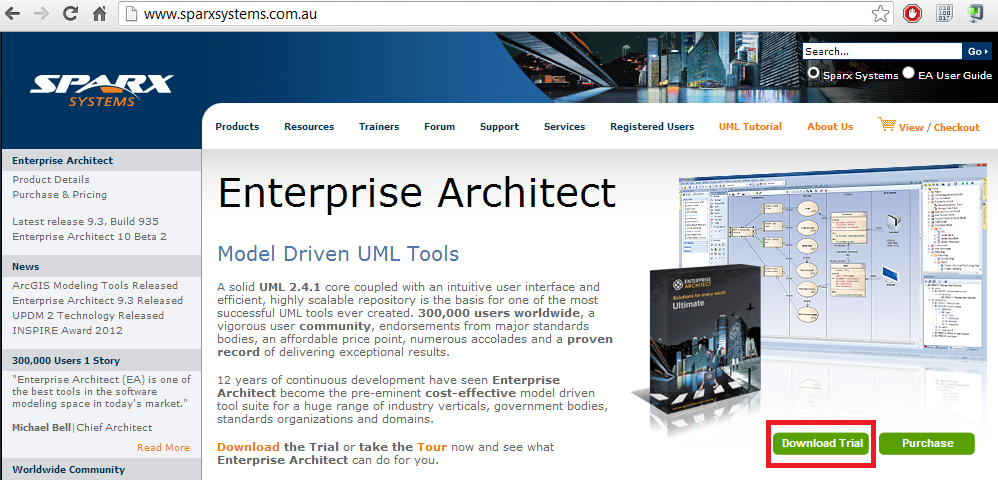
\includegraphics[width=0.77\textwidth]{ea_download}
	\caption{Download Enterprise Architect}
	\label{enterpriseArchitextHomepage}
\end{figure} 

\item Install our EA extension (\Cref{eaPluginWizard}) to add support for our modelling languages.
Download 

{\footnotesize \eMoflonEAAddin}

, unpack, and run the contained \filename{MSI} file.

\begin{figure}[htbp]
	\centering
  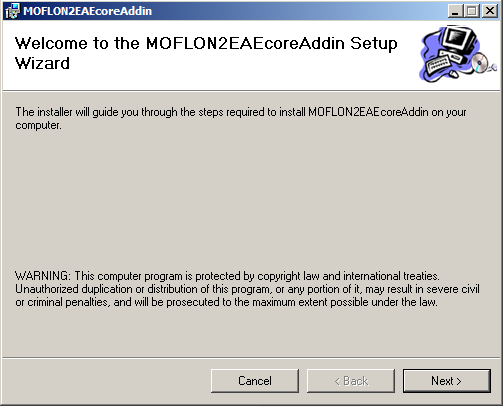
\includegraphics[width=0.55\textwidth]{eaplugin_install}
	\caption{Install our extension for EA}
	\label{eaPluginWizard}
\end{figure}
\end{stepbystep}